\chapter{Introduction}
\label{c:intro}


Letters in math mode will always be in math font, so you must specify text $x=2 and x=3$ is different from $x=2 \text{ and } x=3$. Notice the differential - and use whichever version you are comfortable with.
You can cleverly refer to your equation with \texttt{\textbackslash cref}: \cref{{eq:integration}}.

\section{Figures and Tables}

% Tikzfigure with \input:
\begin{figure}[htbp]
    \centering
    %\documentclass[tikz]{standalone}
%\begin{document}
    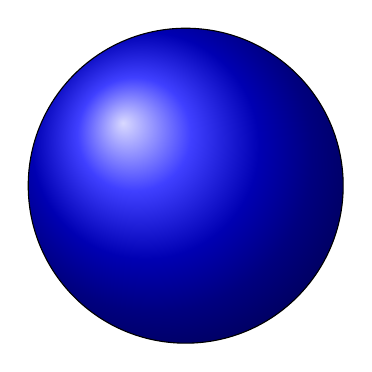
\begin{tikzpicture}
          \draw[shading = ball] (0, 0) circle (2);
    \end{tikzpicture}
%\end{document}
    \caption[One ball]{One ball - and the caption goes underneath the figure.}
\end{figure}

% Includegraphics
\begin{figure}[thbp]
    \centering
    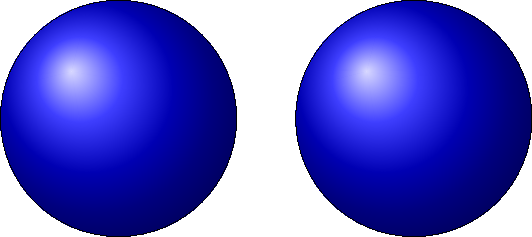
\includegraphics{figures/balls.pdf}
    \caption[Two balls]{Two balls.}
\end{figure}

% Todonotes:
\begin{figure}[hbp]
    \centering
    \missingfigure{Three balls.}
    \caption[Three balls]{Three balls.}
\end{figure}


% Booktabs:
\begin{table}[htbp]
    \centering
       \caption[Colons (to appear in TOC)]{Caption above tables. Proper colon usage.}
    \begin{tabular}{@{}ll@{}}
        \toprule
        \textsf{Correct}               & \textsf{Incorrect}      \\
        \midrule
        \( \varphi \colon X \to Y \)   & \( \varphi : X \to Y \) \\[0.5ex]
        \( \varphi(x) \coloneqq x^2 \) & \( \varphi(x) := x^2 \) \\
        \bottomrule
    \end{tabular}
\end{table}

\begin{table}[htbp]
    \centering
    \caption[Arrows]{Proper arrow usage.}
    \begin{tabular}{@{}ll@{}}
        \toprule
        \textsf{Correct}     & \textsf{Incorrect}         \\
        \midrule
        \( A \implies B \)   & \( A \Rightarrow B \)      \\
        \( A \impliedby B \) & \( A \Leftarrow B \)       \\
        \( A \iff B \)       & \( A \Leftrightarrow B \)  \\
        \bottomrule
    \end{tabular}
    
\end{table}

% Tablefootnote and multirow:
\begin{table}[!ht]
   \caption[Dashes]{Proper dash usage.}
    \centering
    \begin{tabular}{@{}ll@{}}
        \toprule
        \textsf{Correct}
        & 
        \textsf{Incorrect}
        \\
        \midrule
        \( -1 \) 
        & 
        -1
        \\[0.3ex]
        1--10
        &
        1-10
        \\[0.3ex]
        Birch--Swinnerton-Dyer\tablefootnote{It is now easy to tell that Birch and Swinnerton-Dyer are two people, but I don't know why the footnote lands on the wrong page.} conjecture
        &
        Birch-Swinnerton-Dyer conjecture
        \\[0.3ex]
        The ball \dash which is blue \dash is round.
        &
        \multirow{ 2}{*}{The ball - which is blue - is round.}
        \\[0.3ex]
        The ball---which is blue---is round. 
        &
        \\
        \bottomrule
    \end{tabular}
  
\end{table}


\begin{table}[hbtp]
      \caption[Quotation marks]
    {Proper quotation mark usage.
    The \texttt{\textbackslash enquote} command chooses the correct
    quotation marks for the specified language. Moreover, \texttt{\textbackslash resizebox} has been used to control table width.}
    \centering
     \resizebox{\linewidth}{!} {
      \begin{tabular}{@{}*{2}{p{0.5\textwidth}}@{}}
           \toprule
        \textsf{Correct} &  \textsf{Incorrect}
        \\
        \midrule
        \enquote{This is an \enquote{inner quote} inside an outer quote}
        &
        'This is an "inner quote" inside an outer quote'
        \\
        \bottomrule
    \end{tabular}
    }
\end{table}

\section{Outline}

The rest of the text is organised as follows. See more lists in \cref{p1:discussion}.
\begin{description}
    \item[\cref{intro}] consists of an interesting introduction. You could consider calling this a chapter, not a part, but be aware of how this will affect numbering and the table of contents.
    \item[\cref{p1}] is all about your first research problem. The part is subdivided into an IMRaD-structure, starting with \cref{p1:intro}. 
    \item[\cref{p2}] is all about your second research problem. Perhaps you want to reset chapter numbering for each part, but then what would you do with the introduction and conclusion - and how would you ensure unique cross references? See \cref{p1} \cref{p1:intro}.
    \item[\cref{conc}] is your fabulous conclusion. Is this a part? Probably not. But then again you need to think very carefully about numbering.
\end{description}
